% to choose your degree
% please un-comment just one of the following
\documentclass[bsc,twoside,singlespacing,parskip,logo,notimes,normalheadings]{infthesis}
% for BSc, BEng etc.

\usepackage[super]{natbib}
\setcitestyle{square}

\usepackage[toc]{appendix}

\usepackage[acronym,section,numberedsection=autolabel]{glossaries}

\makeglossaries

%% Basics
\newglossaryentry{controlflowgraph}
{
        name=control-flow graph,
        description={A graph representing the possible execution paths
        in a program. Nodes represent instructions, edges represent
        possible jumps between said instructions}
}

\newglossaryentry{dataflowanalysis}
{
        name=data-flow analysis,
        description={A technique for gathering information at various
          points in a \gls{controlflowgraph}}
}
 
\newglossaryentry{dataflow}
{
        name=data-flow,
        description={A system of equations and conditions which
          constitute a data-flow problem, that is, a problem which may
          be solved through data-flow analysis}
}

\newglossaryentry{direction}
{
        name=direction,
        description={The direction in which data flows in a
          \gls{dataflow} problem. Either forward (from the entry point
          of the \gls{cfg} to the exit point) or backward (the opposite)}
}

\newglossaryentry{dataflowequations}
{
        name=data-flow equations,
        description={A system of equations which determine how data
          flows through a \gls{cfg}}
}

\newglossaryentry{transfer}
{
        name=transfer,
        description={An equation (or set of equations) which
          determines how data flows {\em through} a node in a \gls{cfg}}
}

\newglossaryentry{meet}
{
        name=meet,
        description={An equation (or set of equations) which
          determines how data flows {\em between} nodes in a \gls{cfg}}
}

%%Generic Frameworks 
\newglossaryentry{hassediagram}
{
        name=Hasse diagram,
        description={A diagram used to represent partially ordered
          sets. Nodes represent elements of the sets, edges represent
          an ordering between a pair of elements}
}

\newglossaryentry{meetsemilattice}
{
        name=meet semi-lattice,
        description={A partially ordered set in which there exists a
          greatest lower bound (or meet) for any non-empty, finite subset}
}

\newglossaryentry{meetoperator}
{
        name=meet operator,
        description={An operator which defines how the meet of two
          sets is obtained, such as $\cup$, $\cap$ or another operator
        entirely}
}

\newglossaryentry{domain}
{
        name=domain,
        description={The domain of values considered in a
          \gls{dataflow} problem, e.g. definitions or expressions}
}

\newglossaryentry{boundary}
{
        name=boundary,
        description={The initial value at the starting point of an
          analysis, i.e. $\text{In}(ENTRY)$ or $\text{Out}(EXIT)$}
}

\newglossaryentry{fixedpoint}
{
        name=fixed-point,
        description={A computation in which the required process is
          repeated until the state stops changing.}
}



%% Types of Analysis
\newglossaryentry{reachingdefinition}
{
        name=reaching definition,
        description={A definition of a variable 'reaches' a block if there exists at least one path from its definition to the block along which it is not overwritten}
}

\newglossaryentry{livenessanalysis}
{
        name=liveness analysis,
        description={A variable is 'live' if its current value will be used later in the program's execution}
}

\newglossaryentry{availableexpression}
{
        name=available expression,
        description={An expression is 'available' if it has been computed along all paths leading to the current node}
}


 
\newacronym{cfg}{CFG}{control-flow graph}

\usepackage[absolute,overlay]{textpos}
  \setlength{\TPHorizModule}{1mm}
  \setlength{\TPVertModule}{1mm}

\usepackage{tikz}
\usetikzlibrary{arrows.meta,decorations.markings}
\usepackage{wrapfig}
\usepackage{amsmath}
\usepackage{caption}
\usepackage{capt-of}
\usepackage{color}
% \documentclass[minf,frontabs,twoside,singlespacing,parskip,deptreport]{infthesis}  % for MInf

\tikzstyle{block} = [rectangle, draw, text width=6em, text centered, rounded corners, minimum height=1em]
\tikzstyle{set} = [rectangle, text width=6em, text centered, rounded corners, minimum height=1em]
\tikzset{vertex/.style = {shape=circle,draw,minimum size=1.5em}}
\tikzset{edge/.style = {
    >=Stealth,
    -{>[scale=0.8]},
  }
}

\newcommand{\cfgpoint}[1][]{%
  \draw[magenta, fill=magenta!90] (#1) circle (0.5mm);
}

\makeatletter
\renewcommand\NAT@citesuper[3]{\ifNAT@swa
\if*#2*\else#2\NAT@spacechar\fi
\unskip\kern\p@\textsuperscript{\NAT@@open#1\if*#3*\else,\NAT@spacechar#3\fi\NAT@@close}%
   \else #1\fi\endgroup}
\makeatother

\begin{document}

\pagenumbering{roman}

\title{Data-Flow Analysis:\\Simulation and Visualisation}

\author{Ayrton Massey}

% to choose your course
% please un-comment just one of the following
%\course{Artificial Intelligence and Computer Science}
%\course{Artificial Intelligence and Software Engineering}
%\course{Artificial Intelligence and Mathematics}
%\course{Artificial Intelligence and Psychology }   
%\course{Artificial Intelligence with Psychology }   
%\course{Linguistics and Artificial Intelligence}    
\course{Computer Science}
%\course{Software Engineering}
%\course{Computer Science and Electronics}    
%\course{Electronics and Software Engineering}    
%\course{Computer Science and Management Science}    
%\course{Computer Science and Mathematics}
%\course{Computer Science and Physics}  
%\course{Computer Science and Statistics}    

% to choose your report type
% please un-comment just one of the following
%\project{Undergraduate Dissertation} % CS&E, E&SE, AI&L
%\project{Undergraduate Thesis} % AI%Psy
\project{4th Year Project Report}

\date{\today}

\abstract{ \setcounter{page}{1} Data-flow analysis is one of the
  cornerstones of modern compiler optimisation. A thorough
  understanding of the processes involved is essential to further
  exploration of the subject. A tool which allows exploration of
  \gls{dataflowanalysis} in an interactive environment would prove
  invaluable to students encountering the topic for the first time.

  This report describes the design and implementation of an
  interactive system to simulate and visualise forms of data-flow
  analysis on simple assembly-like programs. The system is evaluated
  by in terms of user experience and the achievement of learning
  outcomes, through self-assessment and by examining usage data
  collected during the evaluation period.

  %TODO: Outcome
  The software proved (successful/unsuccessful) in providing a tool
  for increasing the learning capacity of the subjects.
}

\maketitle

\section*{Acknowledgements}
%TODO: Acknowledgements
Acknowledgements go here.

\tableofcontents

%%%%%%%%%%%%%%%%%%%%%%%%%%%%%%%%%%%%%%%
\chapter{Introduction}
\pagenumbering{arabic}

This chapter gives a short introduction to the topic of data-flow
analysis, describes motivations and desired outcomes for the project
and provides a brief summary of contributions.


    \section{Data-Flow Analysis}
    \Gls{dataflowanalysis} is a tool for analysing the flow of data
    through a program at various points in its execution. Analysis is
    performed over a \gls{controlflowgraph}, computing the properties
    of values flowing {\em in} and {\em out} of each node. Many forms
    of data-flow analysis exist to compute various properties, for
    example {\em \gls{livenessanalysis}} identifies variables which
    will be used in future instructions and {\em
      \gls{availableexpression}s} identifies those expressions whose
    value has been previously computed at some point in the
    \gls{controlflowgraph}.
    
    This analysis is used to inform optimisations which can be
    performed on a given program. Using the example of {\em
      \gls{livenessanalysis}}, the values computed can be used to
    optimise register allocation: a variable which is not live at a
    given point does not need to be allocated to a register, enabling
    more efficient use of available resources.
    
    Data-flow analysis is not only useful in compiler
    optimisation. The information gathered can be used in other ways,
    such as identifying unsafe operations in PHP web
    applications\cite{TaintedFlow} by monitoring
    sanitization\footnote{To {\em sanitize} a user input is to remove
      any potentially dangerous elements from said input; for example,
      if a user input string is to be inserted into the HTML of a
      webpage it could be sanitized by replacing instances of {\tt
        \textless} and {\tt \textgreater} with {\tt \&lt;} and {\tt
        \&gt;}, respectively. This would prevent that input being
      misinterpreted as HTML and thus avoid malicious scripts
      contained within that input from being executed.} of variables
    which have been assigned to user input.


    \section{Motivations}
    This project was inspired by the project's supervisor, Hugh
    Leather. The original concept was an online tutor for
    \gls{dataflowanalysis} which would allow users to simulate an
    analysis on simple programs. The user could vary parameters, such
    as the \gls{dataflow} in question or the order in which nodes are
    evaluated, and examine the resulting solution.
    
    As lecturer of the Compiler Optimisations course at the University
    of Edinburgh, Hugh desired a system which could teach students the
    foundations of the course in a more interactive format than
    standard lectures. The system should be suitable for hosting on
    the course web page to make it accessible to all students.
    
    My personal interest in this project stemmed from a desire to use
    my practical skills to increase my capacity for understanding
    theoretical content. As noted in our early discussions, many
    students find it difficult and time consuming to read and
    understand material from the course textbook. Presenting this
    information in such a way that it could be easily digested by even
    a novice to Computer Science provided an exciting challenge.
    
    
    \section{Objectives}
    The main aim of this project was to create an interactive system
    to teach students the basic principles of \gls{dataflowanalysis}
    in compilers.
    
    This would take the form of a web application using visual
    components which could be combined in different ways, for example
    to present a series of tutorials on \gls{dataflowanalysis} or to
    provide a sandbox environment to explore. The content of the
    application would cover a range of topics from the basics of
    \gls{dataflowanalysis} to algorithms and frameworks for solving
    generic \gls{dataflow} problems.
    
    The application would be aimed at students of the Compiler
    Optimisations course and as such would be based on material from
    the course textbook {\em Engineering a Compiler (2nd
      Edition)}\cite{eac} by Keith D. Cooper and Linda Torczon. The
    application could then be extended to cover the topic in more
    depth using content from {\em Compilers: Principles, Techniques
      and Tools, 1st ed.}\cite{dragonbook} by Alfred V. Aho, Ravi
    Sethi and Jeffery D. Ullman.
    
    Users would be able to interact with the system by providing
    simple assembly-like programs, altering parameters of the analysis
    and stepping through a simulation. Elements of the simulation such
    as the current state and the \gls{controlflowgraph} of the program
    would be visualised on-screen and update as the simulation
    progressed. Each of these elements would be linked visually to
    show how the concepts relate.
    
    The application would be tested on real users. It would be
    evaluated in terms of user experience by analysing interactions
    with the system and conducting a user experience
    survey. Achievement of learning outcomes would be assessed by
    examining responses to questions built into the software and
    self-assessment by the user.
    
    \section{Summary of Contributions}
    The final version of the software is capable of the following:
    
    \begin{itemize}
    \item Simulation of pre-defined \gls{dataflow}s using generic
      framework models. (p. )%TODO: Which page?
    \item Simulation of user-defined programs using the
      ILOC\cite[appx.~A]{eac} language from {\em Engineering a
        Compiler}. (p. )%TODO: Which page?
    \item Simulation using the round-robin iterative algorithm (p.
      ) %TODO: Which page?
    \item User-controlled simulation allowing step-by-step, instant or
      automated playback.
    \item Visualisation of the following simulation elements:
      \begin{itemize}
      \item \Gls{controlflowgraph} (p. )%TODO: Which page?
      \item Simulator state incl. currently evaluated node,
        framework etc. (p. )%TODO: Which page?
      \item Table of results displaying data flowing in / out of each
        node.
      \item \Gls{hassediagram} of \gls{meetsemilattice} (p.
        ) %TODO: Which page?
      \end{itemize}
    \item Tutorials covering basics of the topic with interactive
      elements (p. )%TODO: Which page?
    \item Interactive test to assess achievement of learning outcomes
    \end{itemize}

    In addition, I have produced an API to record user interaction
    events modeled on the Google Analytics event tracking system
    (p. ). %TODO: Which page?

    Detailed explanations of the terminology mentioned above can be
    found in chapter \ref{background-chap}. A quick summary of terms
    can be found in the glossary in appendix \ref{glossary}.


%%%%%%%%%%%%%%%%%%%%%%%%%%%%%%%%%%%%%%%
\chapter{Background}
In this chapter I will briefly cover the necessary background
information required to understand this project, both to inform the
reader and to demonstrate my own understanding of the topic.

    \section{Introduction to Data-Flow Analysis}
    Data-flow analysis computes information about data flowing {\em
      in} and {\em out} of each node in a program's
    \gls{controlflowgraph}. Many types of analysis can be performed
    and the information gathered can be used to inform the decisions
    of optimising compilers. A brief list of analyses and their
    purposes can be found in appendix \ref{analysistypes}.
    
        \subsection{Control-flow Graph}

        \begin{textblock}{80}(20,176)
            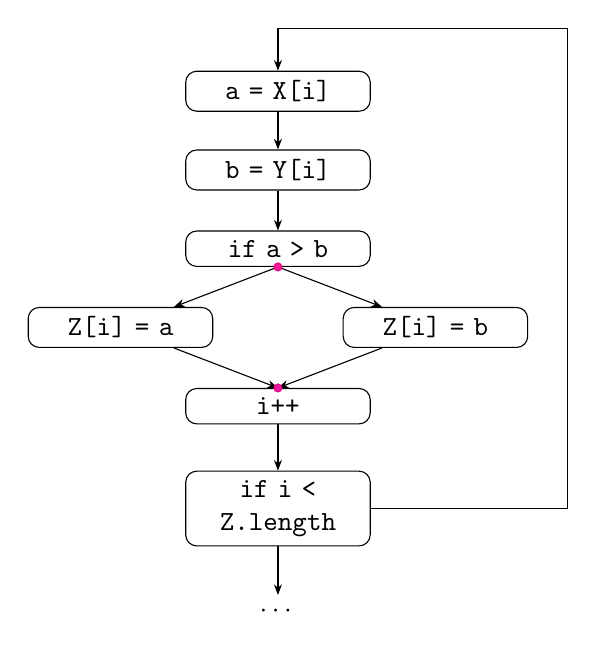
\begin{tikzpicture}[y=-1cm, remember picture]
              % vertices
              \node[block] (n1) at (2 , 0) {\tt a = X[i]};
              \node[block] (n2) at (2 , 1) {\tt b = Y[i]};
              \node[block] (n3) at (2 , 2) {\tt if a > b};
              \node[block] (n4) at (0 , 3) {\tt Z[i] = a};
              \node[block] (n5) at (4 , 3) {\tt Z[i] = b};
              \node[block] (n6) at (2 , 4) {\tt i++};
              \node[block] (n7) at (2 , 5.3) {\tt if i < Z.length};
              \node (n8) at (2 , 6.6) {$\cdots$};
              
              % edges
              \draw[edge] (n1)       to (n2);
              \draw[edge] (n2)       to (n3);
              \draw[edge] (n3.south) to (n4);
              \draw[edge] (n3.south) to (n5);
              \draw[edge] (n4) to (n6.north);
              \draw[edge] (n5) to (n6.north);
              \draw[edge] (n6) to (n7);
              \draw[edge] (n7) to (n8);
              \draw[edge] (n7.east) -| ++(2.5, 0) |- (2.5, -0.8)
              -| (n1.north);

              \cfgpoint[n3.south];
              \cfgpoint[n6.north];
              
            \end{tikzpicture}
            \captionsetup{width=8cm,justification=justified}
            \captionof{figure}{A control-flow graph.}
            \label{cfgexample}
        \end{textblock}

        \hfill\begin{minipage}{\dimexpr\textwidth-6cm}

          A \gls{controlflowgraph} displays the possible execution
          paths for a given program. Each node in the graph represents
          an instruction or basic block, each edge represents an
          execution path leading from that instruction. A node can
          have multiple outward edges if it is a branching
          instruction. Branches may point backward in the
          control-flow. An example of a simple \gls{controlflowgraph}
          can be seen in fig. \ref{cfgexample}.
          
          \vspace{0.26cm}

          A {\em point} in the \gls{controlflowgraph} refers to some
          point along the edges of the graph. In
          \gls{dataflowanalysis} we usually deal with sets of values
          at the {\em in} and {\em out} points of each node, i.e. the
          point where the {\em in-edges} meet and the {\em out-edges}
          originate, respectively (shown in
          \textcolor{magenta}{magenta} on the left).

        \end{minipage}

	\subsection{A Simple Example}
	An oft-used example of \gls{dataflowanalysis} is that of {\em
          \gls{reachingdefinition}s}, which we will demonstrate here due to
        its simplicity. \Gls{reachingdefinition}s computes the set of
        variable definitions which are are available at a given
        point. A definition is said to {\em reach} a point $p$ if
        there is no intermediate assignment to the same variable along
        the path from the definition of the variable to the point $p$.
        
        Let us take the example in fig. \ref{cfgexample}. The first
        node defines the variable {\tt a}. We shall refer to this
        definition of {\tt a} as {\tt a\textsubscript{1}}. The
        definition of {\tt a} reaches each point in the
        \gls{controlflowgraph} as it is never re-defined. The
        definition {\tt c\textsubscript{1}}, however, does not reach
        the exit node as {\tt c} is re-defined by {\tt
          c\textsubscript{2}}. The graph in fig. \ref{rdcfg} shows the
        set of reaching definitions at each point in the program. We
        have combined the {\em in} and {\em out} points to save space.
        
        \begin{wrapfigure}[21]{i}{6.5cm}
          \centering
          \vspace{-5mm}
          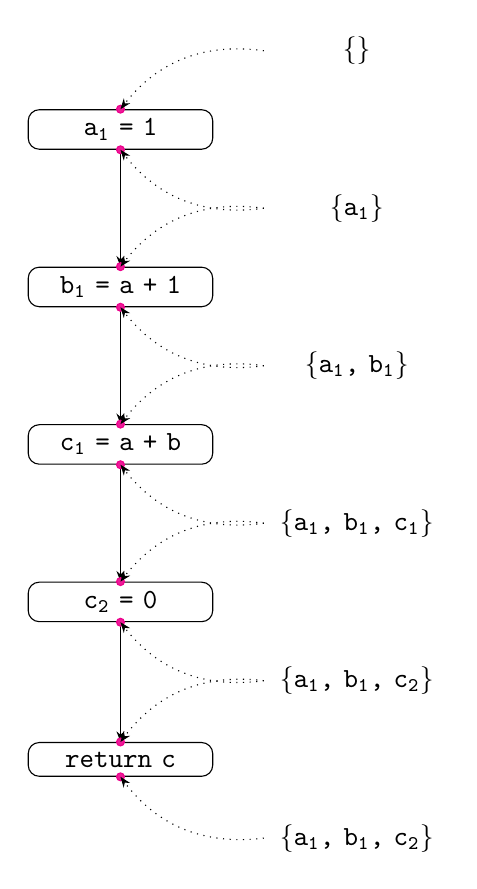
\begin{tikzpicture}[y=-1cm]
            % vertices
       	    \node[set] (s0) at (3 , -1) {\tt \{\}};
            \node[block] (n1) at (0 , 0) {\tt a\textsubscript{1} = 1};
       	    \node[set] (s1) at (3 , 1) {\tt \{a\textsubscript{1}\}};
            \node[block] (n2) at (0 , 2) {\tt b\textsubscript{1} = a + 1};
            \node[set] (s2) at (3 , 3) {\tt \{a\textsubscript{1}, b\textsubscript{1}\}};
            \node[block] (n3) at (0 , 4) {\tt c\textsubscript{1} = a + b};
            \node[set] (s3) at (3 , 5) {\tt \{a\textsubscript{1}, b\textsubscript{1}, c\textsubscript{1}\}};
            \node[block] (n4) at (0 , 6) {\tt c\textsubscript{2} = 0};
            \node[set] (s4) at (3 , 7) {\tt \{a\textsubscript{1}, b\textsubscript{1}, c\textsubscript{2}\}};
            \node[block] (n5) at (0 , 8) {\tt return c};
       	    \node[set] (s5) at (3 , 9) {\tt \{a\textsubscript{1}, b\textsubscript{1}, c\textsubscript{2}\}};
            
            %edges
            \draw[edge] (n1) to (n2);
            \draw[edge] (n2) to (n3);
            \draw[edge] (n3) to (n4);
            \draw[edge] (n4) to (n5);

            \cfgpoint[n1.north]
            \cfgpoint[n1.south]
            \cfgpoint[n2.north]
            \cfgpoint[n2.south]
            \cfgpoint[n3.north]
            \cfgpoint[n3.south]
            \cfgpoint[n4.north]
            \cfgpoint[n4.south]
            \cfgpoint[n5.north]
            \cfgpoint[n5.south]
            
            %set lines
            \draw[edge, dotted] (s1.west) to [bend left] (n1.south);
	    \draw[edge, dotted] (s2.west) to [bend left] (n2.south);
	    \draw[edge, dotted] (s3.west) to [bend left] (n3.south);
	    \draw[edge, dotted] (s4.west) to [bend left] (n4.south);
	    \draw[edge, dotted] (s5.west) to [bend left] (n5.south);
            \draw[edge, dotted] (s0.west) to [bend right] (n1.north);
            \draw[edge, dotted] (s1.west) to [bend right] (n2.north);
	    \draw[edge, dotted] (s2.west) to [bend right] (n3.north);
	    \draw[edge, dotted] (s3.west) to [bend right] (n4.north);
	    \draw[edge, dotted] (s4.west) to [bend right] (n5.north);
            
          \end{tikzpicture}
          \captionsetup{justification=centering}
          \caption{A \gls{controlflowgraph}.}
          \label{rdcfg}
        \end{wrapfigure}
        
        Data-flows have {\em direction}. Reaching definitions is a
        {\em forward flow problem}; values flow from the entry node of
        the \gls{cfg} to the exit node.

        The values at each point are determined using {\em data-flow
          equations}. For example, the equations for reaching
        definitions (defined in terms of {\em in} and {\em out}) at a
        given node $n$ are:
        
        \vspace{-7mm}
        \begin{align*}
          \textnormal{In}(n)  & = \bigcup_{p \in preds} \textnormal{Out}(n) \\
          \textnormal{Out}(n) & = \textnormal{DefGen}(n) \cup (\textnormal{In}(n) \setminus \textnormal{Out}(n))
        \end{align*}
        
        The equations for $\text{In}(n)$ and $\text{Out}(n)$ are often
        referred to as {\em \gls{meet}} and {\em \gls{transfer}}
        functions. In a forward flow problem the meet function
        combines the {\em out} sets of a node's predecessors to form
        its {\em in} set. The \gls{transfer} function computes a
        node's {\em out} set from its {\em in} set and information
        obtained from the node itself, thereby {\em transferring}
        values through a node.

	\subsection{Lattices}
	Sets in a \gls{dataflow} problem have a partial order. This
        can be expressed using a structure known as a {\em
          \gls{meetsemilattice}}. A \gls{meetsemilattice} consists of
        a set of possible values $L$, the meet operator $\land$, and a
        {\em bottom element} $\bot$. The semi-lattice imposes an order
        on values in $L$ such that:
        
        \vspace{-1cm}
        %TODO: REFERENCE
        \begin{align*}
          a \geq b \;\text{if and only if}\; & a \land b = b \\
          a \ge  b \;\text{if and only if}\; & a \land b = b \;\text{and}\; a \neq b
        \end{align*}
        \vspace{-1cm}
        
        For the bottom element $\bot$, we have the following:
        
        \vspace{-1cm}
        %TODO: REFERENCE
        \begin{align*}
          \forall a \in L,\; & a \geq \bot \\
          \forall a \in L,\; & a \land \bot = \bot
        \end{align*}
        \vspace{-1cm}
        
        %TODO: REFERENCE
        We can express the semi-lattice using a {\em \gls{hassediagram}}, shown in fig. \ref{meethasse}.

        \begin{wrapfigure}[12]{o}{7cm}
          \vspace{-5mm}
          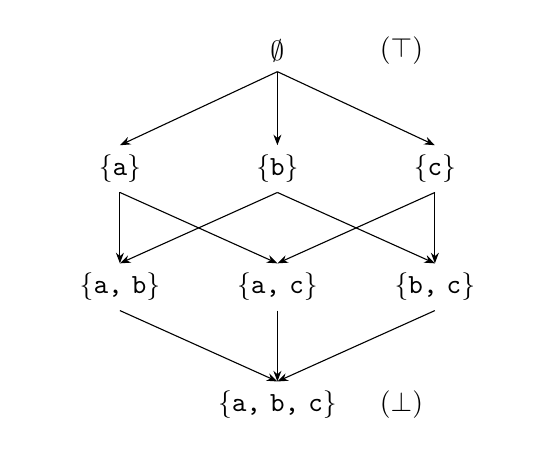
\begin{tikzpicture}[y=-1cm]            
            % vertices
       	    \node[set, label={[distance=1cm]0:$(\top)$}] (s1) at (2 , 0.0) {$\emptyset$};
	    \node[set] (s2) at (0 , 1.5) {\tt \{a\}};
            \node[set] (s3) at (2 , 1.5) {\tt \{b\}};
            \node[set] (s4) at (4 , 1.5) {\tt \{c\}};
	    \node[set] (s5) at (0 , 3.0) {\tt \{a, b\}};
	    \node[set] (s6) at (4 , 3.0) {\tt \{b, c\}};
            \node[set] (s7) at (2 , 3.0) {\tt \{a, c\}};
	    \node[set, label={[distance=1cm]0:$(\bot)$}] (s8) at (2 , 4.5) {\tt \{a, b, c\}};
            
            %set lines
            \draw[edge] (s1.south) -- (s2.north);
            \draw[edge] (s1.south) -- (s3.north);
            \draw[edge] (s1.south) -- (s4.north);
            
            \draw[edge] (s2.south) -- (s5.north);
            \draw[edge] (s2.south) -- (s7.north);
            \draw[edge] (s3.south) -- (s5.north);
            \draw[edge] (s3.south) -- (s6.north);
            \draw[edge] (s4.south) -- (s6.north);
            \draw[edge] (s4.south) -- (s7.north);
            
            \draw[edge] (s5.south) -- (s8.north);
            \draw[edge] (s6.south) -- (s8.north);
            \draw[edge] (s7.south) -- (s8.north);
            
          \end{tikzpicture}
          \captionsetup{width=6cm, justification=centering}
          \caption{A \gls{hassediagram} for the meet function $a \land b = a \cup b$.}
          \label{meethasse}
        \end{wrapfigure}
        
        %TODO: REFERENCE
        Some data-flows deal with sets of pairs of values. In constant
        propagation, we pair a variable with one of three elements:
        $undef (\top)$, $nonconst (\bot)$ and $const$. A variable is
        initially paired with $undef$. When it is assigned a constant
        value, we assign it that value. If it is later assigned
        another value, we assign it $nonconst$. This can be expressed
        as the meet function seen in fig. \ref{constmeet}.
        
        The values form a semi-lattice, as seen in
        fig. \ref{consthasse}.

        \begin{figure}[h]
        \begin{align*}
        nonconst \land c &= nonconst & \text{for any constant} \; c \\
        c \land d &= nonconst &\text{for any constants} \; c \neq d \\
        c \land undef &= c &\text{for any constant} \; c \\
        nonconst \land undef &= nonconst & \\
        x \land x &= x &\text{for any value} \; x
        \end{align*}
        \caption{Equations describing the constant propagation meet function.}
        \label{constmeet}
        \end{figure}
        
        \begin{figure}[b]
          \centering
          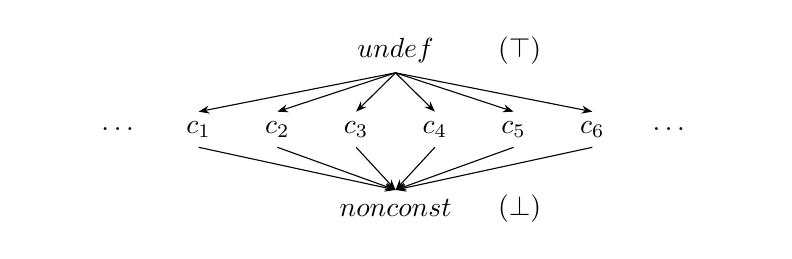
\begin{tikzpicture}[y=-1cm]
            
            % vertices
       	    \node[set, label={[distance=1cm]0:$(\top)$}] (s1) at (3.5 , 0) {$undef$};
            \node[set] (s0) at (0, 1) {$\dots$};
	    \node[set] (s2) at (1 , 1) {$c_1$};
            \node[set] (s3) at (2 , 1) {$c_2$};
            \node[set] (s4) at (3 , 1) {$c_3$};
            \node[set] (s5) at (4 , 1) {$c_4$};
            \node[set] (s6) at (5 , 1) {$c_5$};
       	    \node[set] (s7) at (6, 1) {$c_6$};
            \node[set] (s9) at (7, 1) {$\dots$};
	    \node[set, label={[distance=1cm]0:$(\bot)$}] (s8) at (3.5 , 2) {$nonconst$};
            
            %set lines
            \draw[edge] (s1.south) -- (s2.north);
            \draw[edge] (s1.south) -- (s3.north);
            \draw[edge] (s1.south) -- (s4.north);
            \draw[edge] (s1.south) -- (s5.north);
            \draw[edge] (s1.south) -- (s6.north);
            \draw[edge] (s1.south) -- (s7.north);
            
            \draw[edge] (s2.south) -- (s8.north);
            \draw[edge] (s3.south) -- (s8.north);
            \draw[edge] (s4.south) -- (s8.north);
            \draw[edge] (s5.south) -- (s8.north);
            \draw[edge] (s6.south) -- (s8.north);
            \draw[edge] (s7.south) -- (s8.north);
            
          \end{tikzpicture}
          \caption{A \gls{hassediagram} for the meet function described in fig \ref{constmeet}.}
          \label{consthasse}
        \end{figure}
        
    \pagebreak
    
    \section{Algorithms for Analysis}
    Blah Blah

	\subsection{Iterative Algorithm}
	Blah Blah

    \section{Data-Flow Frameworks}

    It is possible to model \gls{dataflow} problems using a generic
    framework. This allows us to use the same algorithm for multiple
    problems by specifying the following constraints\cite[p. 680]{dragonbook}:

    \begin{itemize}
      \item The {\em \gls{domain}} of values on which to operate;
      \item The {\em \gls{direction}} in which data flows;
      \item A set of {\em \gls{dataflowequations}} including the {\em
          \gls{meetoperator}} $\land$ and the set of {\em
          \gls{transfer} functions} $F$\footnote{The function
          corresponding to a particular node/block $B$ is denoted $F_{B}$};
      \item The {\em \gls{boundary}} value $v_{BOUNDARY}$ specifying
        the value at the entry or exit to the \gls{cfg}; and
      \item The {\em initial value}, $\top$, at each point in the graph.
      \end{itemize}

          \subsection{Algorithm for General Frameworks}

          The following algorithm, adapted from the one in the {\em
            dragon book}\cite[p. 691]{dragonbook} to compute the value
          sets at each node using the elements of our general
          framework:

          \begin{figure}[!ht]
            \centering
            \vspace{-5mm}
            \begin{align*}
              & \text{Transfer}_{BOUNDARY} = v_{BOUNDARY};\\
              & {\bf for} \, ( \text{each block} \: B \: \text{in the CFG} ) \; \text{Transfer}_{B} = \top;\\
              & {\bf while} \, ( \text{changes to any} \: \text{Transfer} \: \text{occur} ) \: \{\\
              & \quad \quad {\bf for} \, (\text{each block} \: B \: \text{in the CFG} ) \: \{\\
              & \quad \quad \quad \quad \text{Meet}_{B} \hspace{0.59cm} = \land_{\text{priors} \, P \, \text{of} \,  B} \, \text{Transfer}_{P};\\
              & \quad \quad \quad \quad \text{Transfer}_{B} = F_{B}(In_{B});\\
              & \quad \quad \}\\
              & \}
            \end{align*}
            \caption{Algorithm for Data-Flow Analysis of General Frameworks}
          \end{figure}

          Instead of referring to the value sets as In and Out as the
          {\em dragon book} does, we may call them \Gls{meet} and
          \Gls{transfer}. This allows us to generalise our algorithm
          to both forward and backward analyses; in the forward
          direction Meet is In, whereas in the backward direction it
          is Out (and vice-versa for Transfer).

          We first initialise the Transfer set using the boundary
          condition, then initialise each node's transfer set to our
          initial value $\top$.

          Next, we perform a \gls{fixedpoint} computation on the
          \gls{cfg}, evaluating each node's \Gls{meet} and
          \Gls{transfer} sets using our \gls{dataflowequations} until
          the sets stop changing.

          The \gls{meet} is taken over a node's {\em priors}: in the
          forward direction, the node's predecessors; in the backward
          direction, the node's successors.

          This algorithm can be applied to any framework. In fact, all
          of the \gls{dataflow} problems in appendix
          \ref{analysistypes} may be solved using this process.

          \subsection{Conditions for Termination}
          
          We must be careful when constructing our general
          frameworks. If our value sets continuously change we may
          never reach a \gls{fixedpoint} and thus our computation will
          never halt.

          To avoid this, our frameworks must satisfy the following
          conditions\cite[p. 684]{dragonbook}:

          \begin{itemize}
          \item The set of \gls{transfer} functions, $F$, contains
            the identity function\footnote{The identity function maps
              its input to its output, i.e. $F(x)=x$};
          \item $F$ is closed under composition: that is, for any two
            functions $f$ and $g$, $f(g(x))$ is also in $F$;
          \item $F$ is monotone; and
          \item The \gls{domain} and the \gls{meetoperator}, $\land$, must
            form a \gls{meetsemilattice}.
          \end{itemize}

          These conditions ensure that during every iteration of the
          algorithm the values at each point will either become {\em
            smaller} (with respect to the partial ordering) or stay
          the same. Since $F$ is monotone, all of the sets must
          eventually stop changing {\bf or} reach the bottom element
          of the lattice, $\bot$, at which point they cannot change
          any further.


%%%%%%%%%%%%%%%%%%%%%%%%%%%%%%%%%%%%%%%
\chapter{Related Work}
Blah Blah

	\section{Compiler Simulation}
	Blah Blah

	\section{Compiler Visualisation}
	Blah Blah

	\section{Interactive Learning Environments}
	Blah Blah


%%%%%%%%%%%%%%%%%%%%%%%%%%%%%%%%%%%%%%%
\chapter{Data-Flow Analysis Simulation}
Blah Blah

	\section{Data-Flow Framework}
	Blah Blah

        \section{Algorithms for Analysis}
	Blah Blah

	\subsection{Iterative Algorithm}
	Blah Blah
    
    	\subsection{Structural Algorithm}
	Blah Blah
        
	\section{Intermediate Language for Optimising Compilers}
	Blah Blah
    
    	\subsection{Parsing Expression Grammar}
	Blah Blah
    
    	\subsection{Control-Flow Graphs}
        Blah Blah


%%%%%%%%%%%%%%%%%%%%%%%%%%%%%%%%%%%%%%%
\chapter{Data-Flow Analysis Visualisation}
Blah Blah

    \section{Data-Flow Framework}
    Blah Blah
    
    \section{Simulator}
    Blah Blah
    
    \section{Control-Flow Graph}
    Blah Blah
    
    \section{Lattice}
    Blah Blah
    

%%%%%%%%%%%%%%%%%%%%%%%%%%%%%%%%%%%%%%%
\chapter{Interactive Learning}

    \section{User-defined Programs}
    Blah Blah
    
    \section{Interactive Tutorials}
    Blah Blah
    
    \section{Experimental Sandbox}
    Blah Blah
    

%%%%%%%%%%%%%%%%%%%%%%%%%%%%%%%%%%%%%%%
\chapter{Evaluation}
Blah Blah


\begin{appendices}

\chapter{Terminology}\label{glossary}

\printglossaries

\chapter{Types of Data-Flow Analysis}\label{analysistypes}

Table \ref{dfatypes} covers a selection of data-flow analyses and lists some of their applications.

\begin{center}
  \begin{tabular}{|l|p{5cm}|p{5cm}|}
    \hline
    {\bf Data-Flow}                         & {\bf Purpose}                                                                                              & {\bf Applications}                                                                              \\ \hline
    Dominators                              & Computes the set of nodes which dominate the current node.                                                 & Computing SSA form.                                                                             \\ \hline
    \Gls{reachingdefinition}s               & Computes the set of variable definitions which are available at points in the CFG.                         & Generating def-use chains for other analyses.                                                   \\ \hline
    \Gls{livenessanalysis}                  & Computes the set of variables whose current value will be used at a later point in the control flow graph. & Register allocation. Identifying useless store operations. Identifying uninitialised variables. \\ \hline
    \Gls{availableexpression}s              & Identifies expressions which been computed at a previous point in the CFG.                                 & Code motion.                                                                                    \\ \hline
    Anticipable Expressions                 & Computes expressions which will be computed along all paths leading from the current point.                & Code motion.                                                                                    \\ \hline
    Constant Propagation                    & Computes the set of variables which have a constant value based on previous assignments.                   & Constant propagation. Dead code elimination.                                                    \\ \hline
    Copy Propagation                        & Computes the set of variables whose values have been copied from another variable.                         & Dead code elimination. Code motion.                                                             \\ \hline
    Tainted Flow Analysis\cite{TaintedFlow} & Identifies unsafe operations which have been passed unsanitized {\em (tainted)} input as a parameter.      & Preventing security vulnerabilities such as SQL injection and XSS attacks.                      \\ \hline
  \end{tabular}
  \captionof{table}{Types of data-flow analysis.}\label{dfatypes}
\end{center}


\end{appendices}

% use the following and \cite{} as above if you use BibTeX
% otherwise generate bibtem entries
\bibliographystyle{unsrtnat}
\bibliography{mybibfile}

\end{document}
